% !TeX TXS-program:compile = txs:///pythonlua

\documentclass[a4paper,11pt]{article}
\usepackage[pythontex]{cp-base}
\graphicspath{{./graphics/}}
%variables
\donnees[%
	typedoc=CHAPITRE~,
	numdoc=1,
	classe=1\up{ère} 2M2,
	matiere={[SPÉ.MATHS]},
	annee=2021,
	titre=Polynômes du second degré
]

%formatage
\author{Pierquet}
\title{\nomfichier}
\hypersetup{%
	pdfauthor={Pierquet},pdftitle={\nomfichier},allbordercolors=white,pdfborder=0 0 0,pdfstartview=FitH}
%divers
\lhead{\entete{\matiere}}
\chead{\entete{\lycee}}
\rhead{\entete{\classe{} - Chapitre \thepart}}
\lfoot{\pied{\matiere}}
\cfoot{\logolycee{}}
\rfoot{\pied{\numeropagetot}}

\begin{document}

\pagestyle{fancy}

\part{CH01 - Polynômes du second degré}

\section{Différentes formes d'écriture}

\subsection{Forme développée réduite}

\begin{cdefi}
On appelle \textbf{polynôme du second degré} ou \textbf{trinôme} une expression de la forme \[ P(x)=ax^2+bx+c\quad \mbox{avec $a, b, c$ des réels fixés tels que $a \neq 0$} \] %
ou toute autre expression qui peut se mettre sous cette forme, qu’on appelle \textbf{forme développée réduite}. 

Les nombres $a, b, c$ sont les \textbf{coefficients} du polynôme.
\end{cdefi}

\begin{crmq}
\textit{Polynôme} signifie \emph{plusieurs monômes}. Un monôme désigne une expression de la forme $ax^n$, où $a\in \R$\ est le \textbf{coefficient} du monôme, et $n \in \N$ est son \textbf{degré}.
\end{crmq}

\begin{cprop}
La courbe représentative d’une telle fonction est toujours une \textbf{parabole}. Elle est  \og {\red ouverte vers le haut} \fg{} (\og souriante \fg) si $a$ est positif, elle est  \og {\blue ouverte vers le bas} \fg{} si $ a $ est négatif.
\end{cprop}

\begin{cillustr}
\begin{center}
	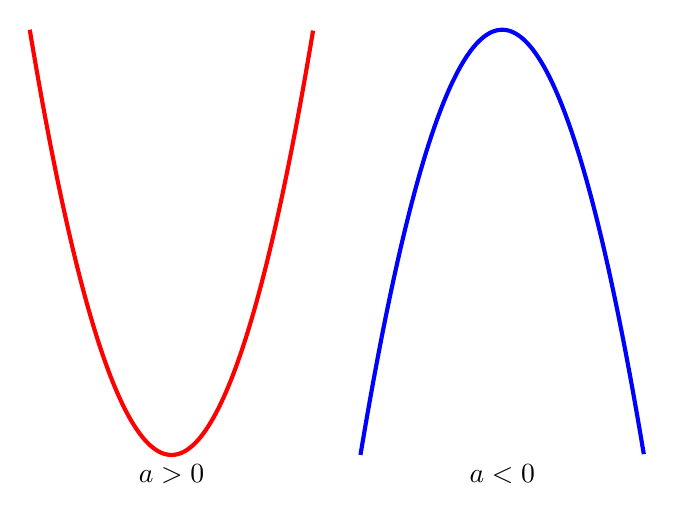
\begin{tikzpicture}[x=0.6 cm,y=0.6 cm]
		\draw[line width=1.5pt,red,domain=-1:5,samples=200] plot (\x,{(\x-2)*(\x-2)-2}) ;
		\draw[line width=1.5pt,blue,domain=6:12,samples=200] plot (\x,{-(\x-9)*(\x-9)+7}) ;
		\draw (2,-2) node[below] {\red $a > 0$} ;
		\draw (9,-2) node[below] {\blue $a < 0$} ;
	\end{tikzpicture}
\end{center}
%{\centering
%\psset{unit=0.6cm,algebraic=true}
%\begin{pspicture}[](-3,-3)(12,7)
%	\psplot[linewidth=1.5pt,linecolor=red]{-1}{5}{(x-2)^2-2}
%	\uput[d](2,-2){\red $a > 0$}
%	\psplot[linewidth=1.5pt,linecolor=blue]{6}{12}{-(x-9)^2+7}
%	\uput[d](9,-2){\blue $a < 0$}
%\end{pspicture}\par}
\end{cillustr}

\subsection{Forme canonique}

\begin{cdefi}
La \textbf{forme canonique} d’un tel polynôme est celle qui s’écrit en utilisant une seule fois la lettre $x$, et qui permet de trouver facilement le \textbf{programme de calcul} de la fonction.

Elle est toujours de la forme $f(x)=a(x-\alpha)^2+\beta $.
\end{cdefi}

\begin{cprop}
Dans la forme canonique $f(x)=a(x-\alpha)^2+\beta$, $a$ est le coefficient de plus haut degré (le même que celui de la forme développée), et $ \alpha $ et $ \beta $ sont les \textbf{coordonnées du sommet} de la parabole qui représente $f$.
\end{cprop}

\begin{cdemo}
\begin{itemize}[leftmargin=*]
	\item Le point $S(\alpha\,;\,\beta)$ est bien un point de la parabole car $f(\alpha)=a \times 0+\beta=\beta$.
	\item Comme $(x-\alpha)^2 \geqslant 0$ pour tout $x \in \R$, alors pour tout $x \in \R$ :
	\begin{center}
		\begin{tabularx}{12cm}{Y|Y}
			si $a>0$ & si $a<0$ \\ 			
			$a(x-\alpha)^2 \geqslant 0$ & $a(x-\alpha)^2 \leqslant 0$ \\ 
			$a(x-\alpha)^2+\beta \geqslant \beta$ & $a(x-\alpha)^2+\beta \leqslant \beta$ \\ 
			$f(x) \geqslant \beta$ & $f(x) \leqslant \beta $ \\
			$\beta$ est le minimum de $f$ & $\beta$ est le maximum de $f$\\
	\end{tabularx} 
	\end{center}
\end{itemize}
\end{cdemo}

\begin{cprop}
Une parabole est symétrique par rapport à la verticale passant par son sommet.
\end{cprop}

\subsection{Forme factorisée}

\begin{cdefi}
Dans certains cas, un polynôme du second degré \textit{peut} aussi s'écrire sous la forme  \[f(x)=a(x-x_1)(x-x_2) \] où $a$ est le coefficient de plus haut degré (le même que celui de la forme développée), et $x_1$ et $x_2$ sont les \textbf{racines} du polynôme.

Cette écriture s'appelle la \textbf{forme factorisée} du polynôme.
\end{cdefi}

\begin{cprop}
Les \textbf{racines} du polynôme sont les valeurs qui annulent le polynôme.

Ce sont les abscisses des \textbf{points d'intersection} de la parabole avec l'axe des abscisses.
\end{cprop}

\begin{chistoire}
\vspace{-0.22cm}
\lettrine[findent=.5em,nindent=0pt,lines=3,image,novskip=0pt]{alkhwarizmi}{}\textit{Mohammed Al-Khwarizmi} (780/850, $\vcenter{\hbox{
\includegraphics[height=0.5\baselineskip]{uzb}}}$) est le premier des mathématiciens persans, et sans doute le plus connu. Il vit à Bagdad du temps de la splendeur de la dynastie abbasside. Le plus célèbre de ses écrits, \textit{Kitâb al-jabr wa al-muqâbala} fut traduit en latin au XII\up{e} siècle, sous le titre \textit{Algebra}. Traitant de la résolution des équations du second degré, il est considéré comme le premier manuel d'algèbre.
\end{chistoire}

\section{Discriminant et racines}

\subsection{Mise sous forme canonique}

\begin{cprop}
Dans la forme canonique, $\alpha$ et $\beta$ se déterminent grâce aux formules suivantes : \[ \alpha=\frac{-b}{2a} \quad \mbox{et} \quad \beta=f(\alpha).\]
\end{cprop}

\begin{cdemo}
On a $f(x)=ax^2+bx+c=a \left(x^2+\frac{b}{a}x+\frac{c}{a}\right)=a\left[ \left(x+\frac{b}{2a} \right)^2-\left(\frac{b}{2a}\right)^2+\frac{c}{a} \right] = a\left[ \left(x+ \frac{b}{2a} \right)^2-\frac{b^2-4ac}{4a^2} \right]$.

\smallskip

On retrouve bien la formule donnée pour $\alpha$ et on a vu plus haut déjà que $f(\alpha)=\beta$.
\end{cdemo}

\begin{calgo}
En \calgpython, on peut créer une \calg{fonction} permettant de calculer les valeurs de $\alpha$ et de $\beta$ :

\begin{tcpythoncode}[15cm]
	\begin{pyverbatim}[][fontsize=\footnotesize,numbers=left,numbersep=10pt]
		# Calcul de alpha et de beta
		from math import *
		def formecanonique(a,b,c):
			alpha = -b/(2*a)
			beta = a*alpha**2 + b*alpha + c
			return alpha, beta
	\end{pyverbatim}
\end{tcpythoncode}

\begin{pyconcode}
# Calcul de alpha et de beta
from math import *
def formecanonique(a,b,c):
	alpha = -b/(2*a)
	beta = a*alpha**2 + b*alpha + c
	return alpha, beta
	

\end{pyconcode}

\begin{consolepython}[15cm]
\begin{pyconsole}[][framesep=3mm,frame=single,label={[\scriptsize Début de la console \logopython]\scriptsize Fin de la console \logopython},fontsize=\footnotesize,framerule=1pt,rulecolor=\color{ForestGreen}]
formecanonique(-3,-5,2)
\end{pyconsole}
\end{consolepython}
\medskip
\end{calgo}

\subsection{Discriminant}

\begin{cdefi}
Soit $f(x)=ax^2+bx+c$ un polynôme du second degré.

On appelle \textbf{discriminant} et on note $\Delta$ le nombre \[\Delta=b^2-4\times a \times c.\]
\end{cdefi}

\begin{cprop}
Le polynôme ne peut être factorisé que si $\Delta$ est positif.
\end{cprop}

\begin{cdemo}
Dans la forme canonique, avec les formules ci-dessus, on a :

$f(x)=a\left[ \left(x+ \frac{b}{2a} \right)^2-\frac{b^2-4ac}{4a^2} \right]=a\left[ \left(x+ \frac{b}{2a} \right)^2-\frac{\Delta}{4a^2} \right]$.

\begin{itemize}[leftmargin=*]
	\item Lorsque $\Delta$ est positif, on voit apparaître dans les crochets une différence de deux carrés, que l'on sait factoriser à l'aide de l'identité remarquable $A^2-B^2=(A-B)(A+B)$ ;
	\item Quand $\Delta$ est  négatif, on y retrouve une somme de deux nombres positifs.
\end{itemize}
\end{cdemo}

\begin{calgo}
En \calgpython, on peut créer une \calg{fonction} permettant de calculer la valeur de $\Delta$ :

\begin{tcpythoncode}[15cm]
	\begin{pyverbatim}[][fontsize=\footnotesize,numbers=left,numbersep=10pt]
		# Calcul de delta
		from math import *
		def delta(a,b,c):
			delta = b**2 -4*a*c
			return delta
	\end{pyverbatim}
\end{tcpythoncode}

\begin{pyconcode}
# Calcul de delta
from math import *
def delta(a,b,c):
	delta = b**2 -4*a*c
	return delta
	

\end{pyconcode}

\begin{consolepython}[15cm]
\begin{pyconsole}[][framesep=3mm,frame=single,label={[\scriptsize Début de la console \logopython]\scriptsize Fin de la console \logopython},fontsize=\footnotesize,framerule=1pt,rulecolor=\color{ForestGreen}]
delta(-3,-5,2)
\end{pyconsole}
\end{consolepython}
\smallskip
\end{calgo}

\subsection{Calcul des racines}

\begin{cthm}
Soit $f(x)=ax^2+bx+c$ un polynôme du second degré. On calcule $\Delta=b^2-4ac$.
\begin{itemize}
	\item Si $\Delta <0$, alors le polynôme n'a \textbf{pas de racine réelle}. Il ne se factorise pas.
	\item Si $\Delta=0$, alors le polynôme a \textbf{une seule racine}, appelée \textbf{racine double}. Elle est égale à $\alpha=\frac{-b}{2a}$.
	
	La forme canonique est également la forme factorisée.
	\item Si $\Delta>0$, alors le polynôme a \textbf{deux racines réelles $x_1$ et $x_2$} que l'on calcule grâce aux formules \[x_1=\frac{-b-\sqrt{\Delta}}{2a} \quad \mbox{et} \quad x_2=\frac{-b+\sqrt{\Delta}}{2a}.\]
\end{itemize}
\end{cthm}

\begin{cdemo}
On a $f(x)=a\left[ \left(x+ \frac{b}{2a} \right)^2-\left(\frac{\sqrt{\Delta}}{2a}\right)^2 \right]=a \left(x+ \frac{b}{2a}-\frac{\sqrt{\Delta}}{2a}\right)\left(x+ \frac{b}{2a}+\frac{\sqrt{\Delta}}{2a}\right)$.

\smallskip

Il suffit de résoudre l'équation $f(x)=0$ pour trouver les racines de $f$.
\end{cdemo}

\begin{calgo}
En \calgpython, on peut créer une \calg{procédure} permettant de calculer les éventuelles racines :

\begin{tcpythoncode}[15cm]
	\begin{pyverbatim}[][fontsize=\footnotesize,numbers=left,numbersep=10pt]
		# Calcul des éventuelles racines
		from math import *
		def racines(a,b,c):
			# Calcul de Delta avec la fonction précédente
			d = delta(a,b,c)
			print(f"Delta={d}")
			if d < 0 :
				print("Aucune racine")
			elif d == 0 :
				print(f"Une racine, {-b/(2*a)}")
			else :
				print(f"Deux racines, {(-b+sqrt(d))/(2*a)} et {(-b-sqrt(d))/(2*a)}")
	\end{pyverbatim}
\end{tcpythoncode}

\begin{pyconcode}
# Calcul des éventuelles racines
from math import *
def racines(a,b,c):
	d = b**2-4*a*c
	print(f"Delta={d}")
	if d < 0 :
		print("Aucune racine")
	elif d == 0 :
		print(f"Une racine, {-b/(2*a)}")
	else :
		print(f"Deux racines, {(-b+sqrt(d))/(2*a)} et {(-b-sqrt(d))/(2*a)}")
	return
	

\end{pyconcode}

\begin{consolepython}[15cm]
\begin{pyconsole}[][framesep=3mm,frame=single,label={[\scriptsize Début de la console \logopython]\scriptsize Fin de la console \logopython},fontsize=\footnotesize,framerule=1pt,rulecolor=\color{ForestGreen}]
racines(-3,-5,2)
racines(1,1,1)
racines(1,-2,1)
\end{pyconsole}
\end{consolepython}
\smallskip
\end{calgo}

\subsection{Résolution d'équations de degré 2}

\begin{cidee}
Jusqu'à maintenant, pour résoudre une équation de degré 2, le seul outil dont on disposait était la \og règle du produit nul \fg{}  : un produit de facteurs est nul ssi l'un au moins des facteurs est nul.

Pour cela, il fallait donc se ramener à quelque chose de \emph{nul} en passant tout dans un seul membre de l'équation, puis à un \emph{produit} en factorisant, ce qui n'était pas toujours possible.

Nous avons désormais la possibilité d'utiliser les formules discriminant/racines au lieu de factoriser, \textbf{à condition} tout de même d'avoir une équation du type $ax^2+bx+c=0$.
\end{cidee}

\begin{chistoire}
Les équations du second degré sont au centre de l'algèbre \textbf{babylonienne}, dès avant le XVIII\up{e} siècle avant JC. La tablette d'argile BM 1390 a été qualifiée de « véritable petit manuel d'algèbre, consacré à l'équation du second degré et aux systèmes d'équations, et donnant les procédures résolutoires fondamentales ».

Au VIII\up{e} siècle, le mathématicien indien \textit{Sridhar Acharya} indique la manière de calculer les deux racines réelles.

Les équations du second degré ont été étudiées systématiquement par \textit{Al-Khwarizmi}.
\end{chistoire}

\begin{cmethode}
Pour résoudre une équation du second degré (c'est-à-dire \og avec des $x^2$ \fg), on peut :
\begin{itemize}
	\item développer ;
	\item tout passer dans le même membre pour avoir $\ldots=0$ ;
	\item calculer $\Delta$ et les éventuelles racines ;
	\item conclure en donnant l'ensemble des solutions (suivant les cas, $\emptyset, \{\alpha\}$ ou $\{x_1\,;\,x_2\}$).
\end{itemize}
\end{cmethode}

\subsection{Somme et produit des racines}

\begin{cprop}
Soit $f(x)=ax^2+bx+c$ un polynôme du second degré ayant deux racines $x_1$ et $x_2$. Alors :
\begin{itemize} 
	\item la somme des racines est égale à $\frac{-b}{a}$ ;
	\item le produit des racines est égal à $\frac{c}{a}$.
\end{itemize}
\end{cprop}

\begin{cdemo}
Il suffit de calculer $x_1+x_2$ et $x_1 \times x_2$ avec les formules des racines !
\end{cdemo}

\begin{crmq}[s]
\begin{itemize}[leftmargin=*]
	\item On a donc $\frac{x_1+x_2}{2}=\frac{-b}{2a}=\alpha$ , autrement dit la moyenne des racines est égale à $\alpha$.
	
	\smallskip
	
	On retrouve ici l'idée de symétrie de la parabole, par rapport à la verticale passant par son sommet. C'est une façon de déterminer $\alpha$ (et donc la forme canonique) directement à partir de la forme factorisée, sans passer par l'étape développée.
	\item Ces propriétés sont intéressantes lorsque l'une des deux racines est une \emph{racine évidente}, c'est-à-dire une racine que l'on peut \emph{voir} (souvent un petit nombre entier). On utilise alors la formule de la somme ou du produit pour déterminer la deuxième racine sans avoir à calculer $\Delta$ (mais dans tous les cas, on peut aussi déterminer les racines avec la méthode habituelle).
\end{itemize}
\end{crmq}

\end{document}